\documentclass{beamer}
\usepackage{graphicx}
\usepackage{hyperref}



\title{Online Outlier Exploration over Large Datasets}
\author{Matthias Hansen \\
        \texttt{matthias.hansen@rwth-aachen.de}}
\date{Data Mining and Multimedia Search}
\institute{RWTH Aachen University}
\begin{document}
\frame{\titlepage}

\begin{frame}{Motivation}
    \centering{Why do Outlier Detection?}
\end{frame}
\section{Outlier Detection}



\begin{frame}{Example: Gaussian Distribution $\mathcal{N}(0,1)$}
    \centering
    \includegraphics<1>[width=.7\textwidth]{images/gaussian.png}
    \includegraphics<2>[width=.7\textwidth]{images/gaussian_lines.png}

    \visible<2>{Within \alert{red} lines $\implies$ inlier.

    Outside \alert{red} lines $\implies$ outlier.}
\end{frame}

\begin{frame}{The Traditional Approach: Statistical Distributions}
    \begin{itemize}
        \item Statistical Distribution of Data must be known.
        \item Linear Runtime.
        \item Distribution can sometimes be Inferred (e.g. using Expectation Maximization).
    \end{itemize}
\end{frame}

\begin{frame}{Counterexample: Geospatial Data}
    \begin{itemize}
        \item OpenStreetMap Data for South America and South Pacific Islands

        \item Roughly 1.3 Gigabytes of Data. (Raw Positions)

        \item Obtained from \texttt{http://download.geofabrik.com}
    \end{itemize}
    \begin{center}
    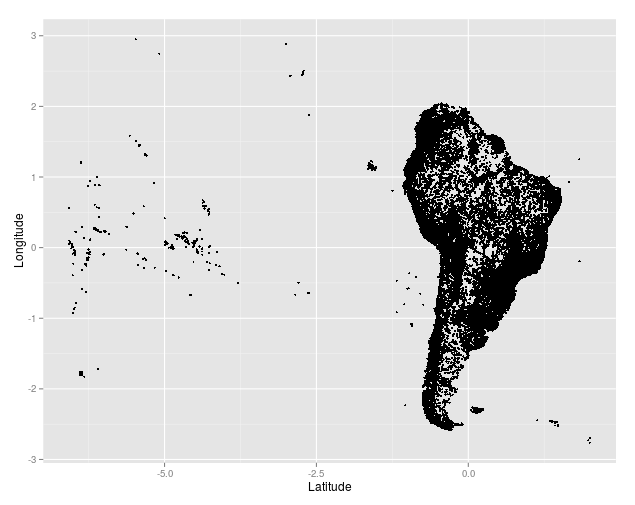
\includegraphics[width=.7\textwidth]{images/south_america.png} 
    \end{center}
\end{frame}

\begin{frame}
    \begin{center}
    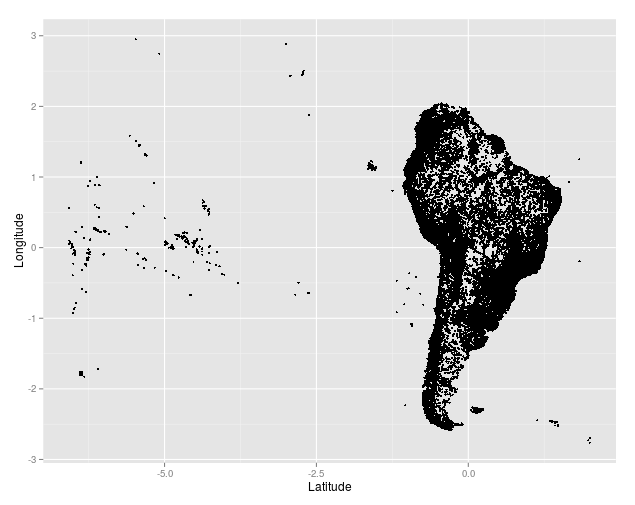
\includegraphics[width=.7\textwidth]{images/south_america.png} 
    \end{center}
    \begin{itemize}
        \item Task: Find wrong data inserted by malicious users.

        \item Example: Someone placed a shop in the middle of the ocean.

    \end{itemize}
\end{frame}

\begin{frame}{Distance-Based Outliers}
    \begin{block}{Distance-Based Outliers}
        Let DB be a sequence of vectors, dist a distance function.

        A point $p\in DB$ is a distance based outlier w.r.t. parameters $k$ and $\varepsilon$
        iff. $|\{q\in DB | dist(p,q) < \varepsilon\}| < k$
    \end{block}

    \begin{itemize}
        \item Same notion as ``non-core points'' in DBSCAN.
        \item Meaningful for geospatial data with Euclidean Distance.
    \end{itemize}
    %TODO add explanatory graphic here
\end{frame}

\section{Outlier Detection and Performance}
\begin{frame}{Performance Considerations}
    \begin{itemize}
        \item Naive way: Calculate pairwise distances. Then check criterion for each point.
        \item Better way: use a spatial Index structure to compute $k$-nearest neighbors. Check whether distance to $k$-th neighbor is $\leq$ $\varepsilon$.
        \item Runtime in $\mathcal{O}(n\log(n))$
    \end{itemize}
\end{frame}

\begin{frame}
    Select some parameters: \visible<2>{\alert{Maybe $k = 5$ and $\varepsilon = 0.0001$?}}
    \begin{center}
        \visible{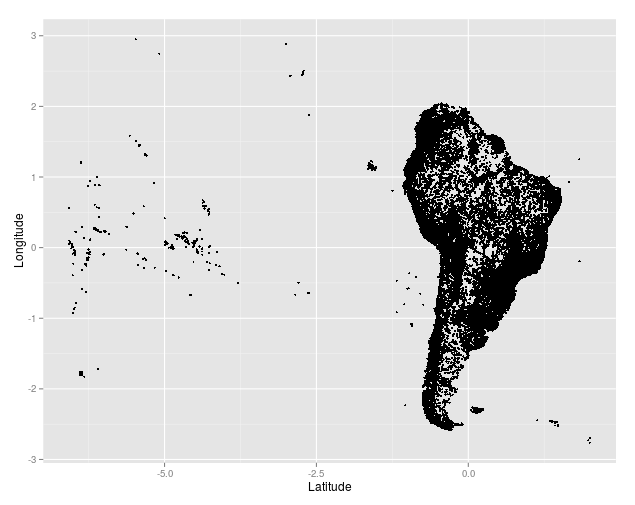
\includegraphics[width=\textwidth]{images/south_america.png}}
    \end{center}
\end{frame}

\begin{frame}
    Select some parameters: \alert{Maybe $k = 5$ and $\varepsilon = 0.0001$}?
    \begin{center}
        \visible{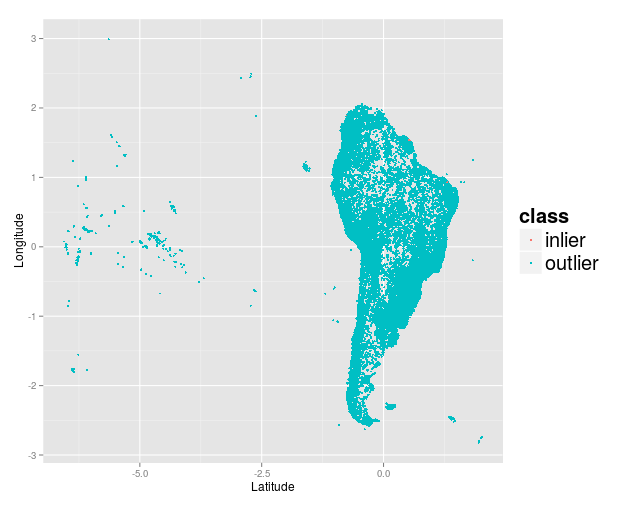
\includegraphics[width=\textwidth]{images/south_america_outliers.png}}
    \end{center}
\end{frame}

\begin{frame}{Parameter Selection is a Problem}
    \begin{itemize}
        \item Good parameter setting not obvious. 
        \item Settings can not be tested on Subsets: \alert{Results will differ!}
        \item Solution?\pause
        \item Use Intermediate Results to support additional faster queries!
    \end{itemize}
\end{frame}


\begin{frame}{A Small Example}

\end{frame}
\end{document}
